\documentclass{eic-bcc-tcc}

%-----------------------------------------------
% Metadados do Trabalho
%-----------------------------------------------
\title{Hedge-fund-lab: Laboratório Quantitativo de Backtesting baseado em Sistemas Multiagentes}
\titleen{Hedge-fund-lab: Quantitative Backtesting Laboratory based on Multi-agent Systems}

% Nome completo dos autores
\addstudent[Lucas Pereira da Silva]{Lucas Pereira da Silva}
\addstudent[Matheus Pereira de Carvalho]{Matheus Pereira de Carvalho}

% Nome do Orientador e titulação (Ajuste o nome se necessário)
\advisor[m]{Nome do Orientador, D.Sc.}

% Ano da defesa do TCC 1
\date{2026}

%-----------------------------------------------
% Abreviações e Acrônimos
%-----------------------------------------------
\newacronym{tcc}{TCC}{Trabalho de Conclusão de Curso}
\newacronym{llm}{LLM}{Large Language Model}
\newacronym{etl}{ETL}{Extract, Transform, Load}
\newacronym{emh}{EMH}{Efficient Market Hypothesis}
\newacronym{amh}{AMH}{Adaptive Markets Hypothesis}
\newacronym{mas}{MAS}{Multi-Agent Systems}
\newacronym{rsi}{RSI}{Relative Strength Index}
\newacronym{sma}{SMA}{Simple Moving Average}

\begin{document}

%-----------------------------------------------
% Elementos Pré-Textuais Automáticos
%-----------------------------------------------
\maketitle

% Como esta é a entrega do TCC 1, os blocos opcionais abaixo podem ser editados depois
\begin{dedicatoria}
Dedicatória opcional dos autores para familiares, amigos e mentores que apoiaram a jornada acadêmica.
\end{dedicatoria}

\begin{agradecimentos}
Agradecimentos opcionais a professores, colegas de curso e instituições que contribuíram diretamente para a realização deste trabalho.
\end{agradecimentos}

\makeapproval

\begin{resumo}
O mercado financeiro contemporâneo caracteriza-se por sua extrema complexidade e natureza não estacionária, onde o volume massivo de dados gerados diariamente desafia as capacidades de análise humana e de algoritmos estáticos tradicionais. Este trabalho apresenta o desenvolvimento do Hedge-fund-lab, um laboratório quantitativo escalável para backtesting de estratégias de investimento baseado em sistemas multiagentes. O objetivo principal é mitigar as limitações de estratégias clássicas e o risco de superajuste através da introdução de processos de debate e consenso na tomada de decisão financeira baseada em Inteligência Artificial. A metodologia compreende a modelagem de uma esteira de dados relacional orquestrada via Prefect e a coordenação de um comitê de agentes especializados utilizando o framework LangGraph. Espera-se demonstrar que a supervisão qualitativa e a deliberação adaptativa de modelos de linguagem reduzem os riscos operacionais em ativos de alta volatilidade do mercado brasileiro.
\palavraschave{Análise Quantitativa. Sistemas Multiagentes. Large Language Models. LangGraph. Backtesting.}
\end{resumo}

\begin{abstract}
The contemporary financial market is characterized by extreme complexity and a non-stationary nature, where the massive volume of data generated daily challenges human analysis and traditional static algorithms. This work presents the development of the Hedge-fund-lab, a scalable quantitative laboratory for backtesting investment strategies based on multi-agent systems. The main objective is to mitigate the limitations of classic trading strategies and the risk of overfitting by introducing debate and consensus processes into financial decision-making driven by Artificial Intelligence. The methodology comprises modeling a relational data pipeline orchestrated via Prefect and coordinating a committee of specialized agents using the LangGraph framework. It is expected to demonstrate that qualitative supervision and adaptive deliberation of large language models reduce operational risks in highly volatile assets within the Brazilian market.
\keywords{Quantitative Analysis. Multi-Agent Systems. Large Language Models. LangGraph. Backtesting.}
\end{abstract>

% Listas e Sumário gerados automaticamente pelo arquivo de classe
\listoffigurespage
\listoftablespage
\listofacronymspage
\tableofcontentspage

%-----------------------------------------------
% Elementos Textuais
%-----------------------------------------------
\mainmatter

\chapter{Introdução}
\label{cha:introducao}

O mercado financeiro contemporâneo caracteriza-se por sua extrema complexidade e natureza não estacionária, onde o volume massivo de dados gerados diariamente desafia as capacidades de análise humana e de algoritmos estáticos tradicionais. No contexto brasileiro, ativos de alta liquidez e volatilidade, como a Petrobras (PETR4) e a WEG (WEGE3), exemplificam como fatores macroeconômicos, decisões políticas e sentimentos de mercado podem alterar drasticamente as tendências de preços em curtos intervalos de tempo. A motivação para este trabalho reside na necessidade de sistemas de apoio à decisão que não apenas processem indicadores técnicos quantitativos, mas que também consigam mimetizar o raciocínio crítico e a adaptação contextual necessária para operar em ambientes de incerteza.

O problema central abordado nesta pesquisa refere-se às limitações das estratégias clássicas de investimento, como o cruzamento de médias móveis e as Bandas de Bollinger, que frequentemente sofrem de superajuste (\textit{overfitting}) ou falham em capturar nuances qualitativas do mercado. O desafio reside em como integrar a robustez da engenharia de dados com a flexibilidade da inteligência artificial generativa para criar um ambiente de simulação que minimize riscos e otimize a alocação de ativos. Surge, então, a questão de como sistemas baseados em \textit{Large Language Models} (LLMs) organizados em uma estrutura multiagente podem superar modelos matemáticos puros ao introduzir processos de debate e consenso na tomada de decisão financeira.

Este trabalho tem como objetivo geral desenvolver o Hedge-fund-lab, um laboratório quantitativo escalável para backtesting de estratégias de investimento baseado em sistemas multiagentes. Para atingir essa meta, definem-se como objetivos específicos: a implementação de um pipeline de dados resiliente utilizando o orquestrador Prefect e o banco de dados PostgreSQL; a construção de um grafo de decisão via LangGraph para coordenar agentes especializados em análise técnica, gestão de risco e análise de sentimento; e, por fim, a realização de testes comparativos entre a performance do sistema multiagente e estratégias clássicas de negociação. Espera-se que a colaboração entre agentes inteligentes permita uma navegação mais segura em cenários de alta volatilidade, validando a eficácia de arquiteturas adaptativas no mercado financeiro.

A presente monografia está organizada em quatro capítulos principais. Além desta introdução, o capítulo 2 apresenta a fundamentação teórica, abordando as hipóteses de eficiência de mercado, as estratégias de análise técnica e a literatura sobre modelos de linguagem e sistemas multiagentes. O capítulo 3 descreve o desenvolvimento da solução, detalhando a modelagem do banco de dados, o fluxo de orquestração e a arquitetura do comitê de agentes. Por fim, o capítulo 4 apresenta as considerações parciais, a metodologia de avaliação experimental e o cronograma de atividades previsto para a conclusão do projeto.


\chapter{Fundamentação Teórica}
\label{cha:fundamentacao}

\section{HIPÓTESE DE EFICIÊNCIA DE MERCADO}

A Hipótese de Eficiência de Mercado (\textit{Efficient Market Hypothesis} -- EMH), formalizada por \citep{Fama1970}, postula que os preços dos ativos financeiros refletem integralmente todas as informações disponíveis. Consequentemente, não seria possível obter retornos anormais de forma consistente utilizando exclusivamente informações públicas ou históricas, uma vez que tais dados já estariam incorporados aos preços.

Fama \citep{Fama1970} classifica a eficiência de mercado em três níveis:

\begin{itemize}
\item Forma fraca: os preços refletem apenas informações históricas de preço e volume;
\item Forma semi-forte: os preços incorporam todas as informações públicas disponíveis;
\item Forma forte: os preços refletem todas as informações, inclusive as privadas.
\end{itemize}

A relevância dessa hipótese para o presente trabalho reside no debate sobre a previsibilidade dos retornos financeiros. Em um mercado perfeitamente eficiente, estratégias quantitativas baseadas em padrões históricos não seriam capazes de gerar retornos superiores de forma consistente. Contudo, evidências empíricas apontam para a existência de anomalias de mercado, como os efeitos momentum e value premium \citep{FamaFrench1992, JegadeeshTitman1993}.

\subsection{Críticas Comportamentais e a Hipótese de Mercados Adaptativos}

Apesar de sua relevância teórica, a EMH recebeu críticas substanciais da economia comportamental. Estudos de \citep{Shiller2000} e \citep{Thaler1993} demonstram que vieses cognitivos, como excesso de confiança, aversão à perda e comportamento de manada, podem levar a desvios persistentes entre preços de mercado e valores fundamentais.

Buscando reconciliar a racionalidade da EMH com as evidências comportamentais, \citet{Lo2004} propôs a Hipótese de Mercados Adaptativos (\textit{Adaptive Markets Hypothesis} -- AMH). Neste modelo, a eficiência de mercado não é um estado fixo, mas um processo dinâmico que evolui ao longo do tempo conforme os agentes aprendem e se adaptam às mudanças no ambiente econômico.

Essa perspectiva fornece suporte teórico para o uso de sistemas baseados em inteligência artificial e modelos de linguagem, uma vez que modelos adaptativos e multiagentes podem capturar padrões dinâmicos e interpretar contextos que estratégias estáticas ou puramente matemáticas não conseguem identificar.

\section{ESTRATÉGIAS BASEADAS EM ANÁLISE TÉCNICA}

A análise técnica assume que padrões históricos de preços e indicadores derivados dessas séries temporais podem gerar sinais úteis para previsão de movimentos futuros do mercado. As estratégias podem ser classificadas em dois grupos principais: estratégias de continuidade de tendência e estratégias de reversão à média.

\subsection{Estratégias de Tendência (Trend Following)}

Estratégias de \textit{trend following} buscam explorar a persistência de movimentos de preço. Evidências empíricas indicam que ativos com bom desempenho recente tendem a continuar apresentando retornos positivos no curto e médio prazo \citep{Moskowitz2012}.

O \textit{Moving Average Crossover} é uma das regras mais estudadas na literatura de análise técnica. \citep{Brock1992} demonstram que regras baseadas em médias móveis apresentam poder preditivo estatisticamente significativo. A média móvel simples é definida como:

\begin{equation}
MA_t = \frac{1}{n} \sum_{i=0}^{n-1} P_{t-i}
\end{equation}

Outra medida amplamente utilizada é o momentum, definido como o retorno acumulado em uma janela temporal:

\begin{equation}
Momentum_t = \frac{P_t}{P_{t-n}} - 1
\end{equation}

\citet{JegadeeshTitman1993} mostram que estratégias baseadas em momentum produzem retornos anormais positivos em horizontes de 3 a 12 meses.

\subsection{Estratégias de Reversão à Média (Mean Reversion)}

A hipótese de reversão à média assume que preços extremos tendem a retornar ao seu valor médio ao longo do tempo. \citep{PoterbaSummers1988} encontram evidências de reversão à média em horizontes de longo prazo. O sinal de negociação pode ser obtido por meio do z-score:

\begin{equation}
z_t = \frac{P_t - \mu}{\sigma}
\end{equation}

onde $\mu$ representa a média móvel e $\sigma$ o desvio padrão.

Entre os indicadores mais utilizados destacam-se o Índice de Força Relativa (RSI), proposto por \citep{Wilder1978}, e as Bandas de Bollinger, introduzidas por \citep{Bollinger2001}. As Bandas de Bollinger são definidas por:

\begin{equation}
BB_{upper} = MA + k\sigma
\end{equation}

\begin{equation}
BB_{lower} = MA - k\sigma
\end{equation}

\section{FACTOR INVESTING E MODELOS DE PRECIFICAÇÃO DE ATIVOS}

Enquanto a análise técnica foca em padrões históricos de preços, o \textit{Factor Investing} busca explicar retornos a partir de características fundamentais das empresas. O modelo de três fatores de \citep{FamaFrench1993} é um dos mais influentes:

\begin{equation}
R_i - R_f = \beta_m (R_m - R_f) + \beta_s SMB + \beta_v HML
\end{equation}

Posteriormente, \citep{FamaFrench2015} expandiram o modelo, adicionando fatores relacionados à rentabilidade e investimento. Estudos recentes demonstram que modelos de \textit{machine learning} podem capturar relações não lineares entre fatores de risco e retornos esperados, superando abordagens lineares tradicionais \citep{Gu2020}.

\section{TEORIA MODERNA DE PORTFÓLIO}

A Teoria Moderna de Portfólio, introduzida por \citep{Markowitz1952}, demonstra que a diversificação permite reduzir o risco total do portfólio sem necessariamente reduzir o retorno esperado. O risco de um portfólio é definido pela variância:

\begin{equation}
\sigma_p^2 = w^T \Sigma w
\end{equation}

Estratégias de alocação derivadas desta teoria incluem \textit{equal weight}, \textit{minimum variance} \citep{Clarke2006} e \textit{risk parity} \citep{Qian2005}. A inclusão de custos de transação é essencial para evitar superestimação de desempenho, especialmente em estratégias com alto \textit{turnover} \citep{LopezDePrado2018}.

\section{SISTEMAS MULTIAGENTES E MODELOS DE LINGUAGEM EM FINANÇAS}

A evolução da Inteligência Artificial Generativa permitiu a aplicação de \textit{Large Language Models} (LLMs) em domínios complexos como o mercado financeiro. Diferente de abordagens baseadas puramente em aprendizado por reforço, sistemas de LLMs utilizam o raciocínio lógico e o processamento de dados não estruturados para a tomada de decisão adaptativa.

\subsection{Arquitetura Multiagente e Raciocínio Colaborativo}

Sistemas multiagentes (\textit{Multi-Agent Systems} -- MAS) operam através da simulação de um comitê de especialistas com funções distintas. No contexto de gestão de portfólio, essa arquitetura permite a divisão de responsabilidades entre agentes especializados, como analistas técnicos, gestores de risco e analistas fundamentalistas.

A utilização de grafos de decisão, através de frameworks como LangGraph, possibilita a implementação de um fluxo de debate. Este processo de consenso visa reduzir o risco de alucinações e combater o fenômeno de \textit{overfitting}, ao exigir que sinais quantitativos sejam validados sob a ótica de risco e contexto macroeconômico. A arquitetura multiagente atua como um sistema de controle e balanço, onde o veredito final de alocação resulta de um processo de raciocínio encadeado (\textit{Chain of Thought}) e deliberação entre as partes.

\section{RISCOS METODOLÓGICOS: OVERFITTING E DATA SNOOPING}

Estratégias quantitativas estão sujeitas ao risco de \textit{overfitting}, especialmente quando múltiplos parâmetros são testados no mesmo conjunto de dados. \citep{Bailey2014} demonstram que a probabilidade de encontrar estratégias aparentemente lucrativas aumenta significativamente quando muitos modelos são testados simultaneamente.

Este fenômeno, conhecido como \textit{data snooping bias}, pode levar a resultados inflados artificialmente. A literatura recomenda validação \textit{out-of-sample}, \textit{walk-forward analysis} e penalizações estatísticas para reduzir esse problema.

\section{MÉTRICAS DE AVALIAÇÃO}

As estratégias serão avaliadas por métricas amplamente utilizadas na literatura financeira. O \textit{Sharpe ratio} \citep{Sharpe1966} é definido como:

\begin{equation}
S = \frac{E[R_p - R_f]}{\sigma_p}
\end{equation}

O \textit{Sortino ratio} \citep{Sortino1994} considera apenas volatilidade negativa. O \textit{Maximum Drawdown} mede a maior perda acumulada durante o período analisado \citep{Magdon2004}. O retorno acumulado é definido por:

\begin{equation}
R_{acum} = \prod_{t=1}^{T} (1 + R_t) - 1
\end{equation}


\chapter{Trabalhos Relacionados}
\label{cha:relacionados}

\section{REVISÃO CRÍTICA DA LITERATURA}

A interseção entre modelos de linguagem e finanças tem sido alvo de crescentes investigações, especialmente no que tange à superação de modelos estáticos. A literatura recente destaca que, embora abordagens baseadas puramente em aprendizado por reforço profundo sejam eficazes, eles apresentam desafios de interpretabilidade e estabilidade em mercados não estacionários \citep{Jiang2017}. Em contrapartida, o uso de técnicas de \textit{machine learning} para capturar relações não lineares em ativos financeiros tem demonstrado resultados superiores às abordagens lineares tradicionais \citep{Gu2020}.

No contexto de sistemas multiagentes, a divisão de responsabilidades entre especialistas — como analistas técnicos e gestores de risco — permite uma mitigação mais eficiente do viés de sobrevivência e do \textit{overfitting} \citep{LopezDePrado2018}. O \textit{Hedge-fund-lab} diferencia-se de soluções genéricas ao propor uma infraestrutura de orquestração resiliente via Prefect, focada especificamente em ativos de alta volatilidade do mercado brasileiro, como PETR4 e WEGE3. 

Enquanto a maioria dos trabalhos relacionados foca em agentes de decisão única ou em redes neurais de caixa-preta, esta pesquisa avança ao implementar um grafo de decisão via LangGraph. Essa arquitetura permite o raciocínio encadeado (\textit{Chain of Thought}) e um processo de debate que simula a governança de um fundo de investimento real, garantindo que as métricas de risco \citep{Bailey2014} sejam verificadas antes de qualquer execução de ordem.

\subsection{Síntese e Hipóteses da Pesquisa}

Com base no referencial teórico apresentado, formulam-se as seguintes hipóteses:

\begin{itemize}
\item \textbf{H1:} Estratégias baseadas em momentum e trend following apresentam desempenho superior ao equal weight em termos de Sharpe ratio.
\item \textbf{H2:} O modelo baseado em um sistema multiagente de LLMs apresenta desempenho superior ajustado ao risco devido à sua capacidade de deliberação adaptativa e mitigação de vieses técnicos.
\item \textbf{H0:} Não há diferença estatisticamente significativa entre as abordagens.
\end{itemize}


\chapter{Método e Desenvolvimento}
\label{cha:metodo}

Este capítulo detalha a modelagem e a elaboração da solução proposta para o Hedge-fund-lab. O desenvolvimento foca na construção de uma infraestrutura que permita a simulação de estratégias de investimento com alta fidelidade, integrando engenharia de dados robusta e inteligência artificial.

\section{ARQUITETURA DO PIPELINE DE DADOS E EXTRAÇÃO}

Para que o comitê de agentes de Inteligência Artificial possa operar em um ambiente simulado, foi desenvolvida uma esteira de dados (Pipeline ETL) resiliente e automatizada. O fluxo de informações foi projetado para capturar, limpar e armazenar dez anos de histórico de negociações de ativos da B3 (especificamente PETR4 e WEGE3), além de calcular os indicadores técnicos que servem de base para a análise comparativa.

A arquitetura utiliza Python como linguagem base, integrando a biblioteca \textit{yfinance} para a ingestão de dados, o banco de dados PostgreSQL para o armazenamento estruturado e o framework Prefect para a orquestração das tarefas.

\subsection{Modelagem do Banco de Dados (PostgreSQL)}

O armazenamento foi desenhado utilizando uma abordagem relacional para garantir a integridade do histórico de preços. A estrutura lógica do banco de dados é dividida nas seguintes tabelas principais:

\begin{itemize}
    \item \textbf{Tabela ativos:} Armazena os metadados das empresas analisadas, incluindo ticker e setor.
    \item \textbf{Tabela cotacoes\_diarias:} Registra o comportamento diário do ativo (abertura, máxima, mínima, fechamento e volume).
    \item \textbf{Tabela indicadores\_tecnicos:} Armazena os cálculos pré-processados de SMA (50 e 200 períodos) e Bandas de Bollinger, evitando gargalos computacionais durante a execução dos agentes.
\end{itemize}

\subsection{Orquestração e Resiliência (Prefect)}

O fluxo de processamento de dados (\textit{Flow}) é orquestrado pelo Prefect para garantir a observabilidade do sistema. O processo é dividido em três tarefas principais:

\begin{enumerate}
    \item \textbf{Extração:} Conecta-se à API financeira para realizar o download da série histórica, com política de tentativas automáticas (\textit{retries}) em caso de falha.
    \item \textbf{Transformação:} Realiza a limpeza de dados nulos e utiliza a biblioteca \textit{pandas} para aplicar as fórmulas matemáticas dos indicadores técnicos.
    \item \textbf{Carga:} Estabelece a conexão com o PostgreSQL e insere os registros em lote (\textit{batch insert}), garantindo a persistência do histórico completo.
\end{enumerate}

\begin{figure}[H]
    \centering
    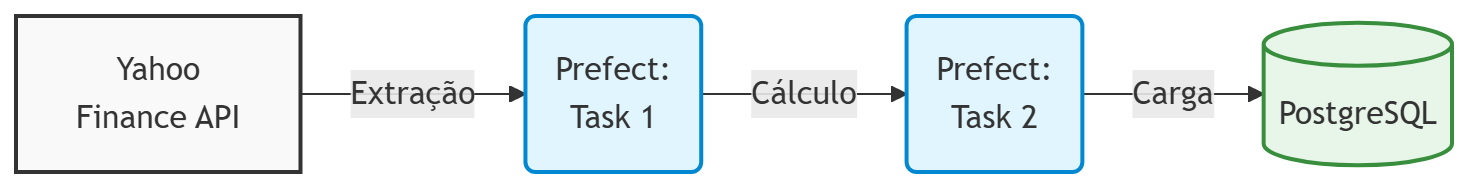
\includegraphics[width=1.0\textwidth]{images/pipeline-etl.png}
    \caption{Fluxo de processamento de dados (ETL) orquestrado pelo Prefect.}
    \label{fig:pipeline_etl}
\end{figure}

\section{ARQUITETURA DO SISTEMA MULTIAGENTES (LANGGRAPH)}

A lógica de decisão do Hedge-fund-lab afasta-se de modelos lineares ao implementar um sistema de agentes autónomos coordenados por um grafo de decisão. Utilizando o framework LangGraph, a tomada de decisão é modelada como um fluxo de estados, onde cada nó representa um agente especializado e as arestas definem as condições de transição entre eles.

\subsection{Modelagem do Grafo de Decisão}

O processo de investimento é estruturado como um debate cíclico ou sequencial, garantindo que nenhuma ordem de compra ou venda seja executada sem uma verificação multicritério. Os principais elements do grafo incluem:

\begin{itemize}
    \item \textbf{Estado do Grafo (State):} Uma estrutura de dados partilhada que armazena o histórico do pregão atual, os sinais gerados pelos analistas, o saldo em caixa e a decisão final.
    \item \textbf{Nó Analista Técnico:} Este agente processa os indicadores quantitativos (Bandas de Bollinger e SMA) recuperados do banco de dados e emite uma recomendação inicial.
    \item \textbf{Nó Gestor de Risco:} Atua como um filtro crítico, avaliando a volatilidade do ativo e o impacto da operação no património total, possuindo autoridade para vetar decisões do analista.
    \item \textbf{Nó Gestor de Portfólio:} Responsável por consolidar as análises e determinar o volume exato da operação, finalizando o estado do grafo para execução.
\end{itemize}

\begin{figure}[H]
    \centering
    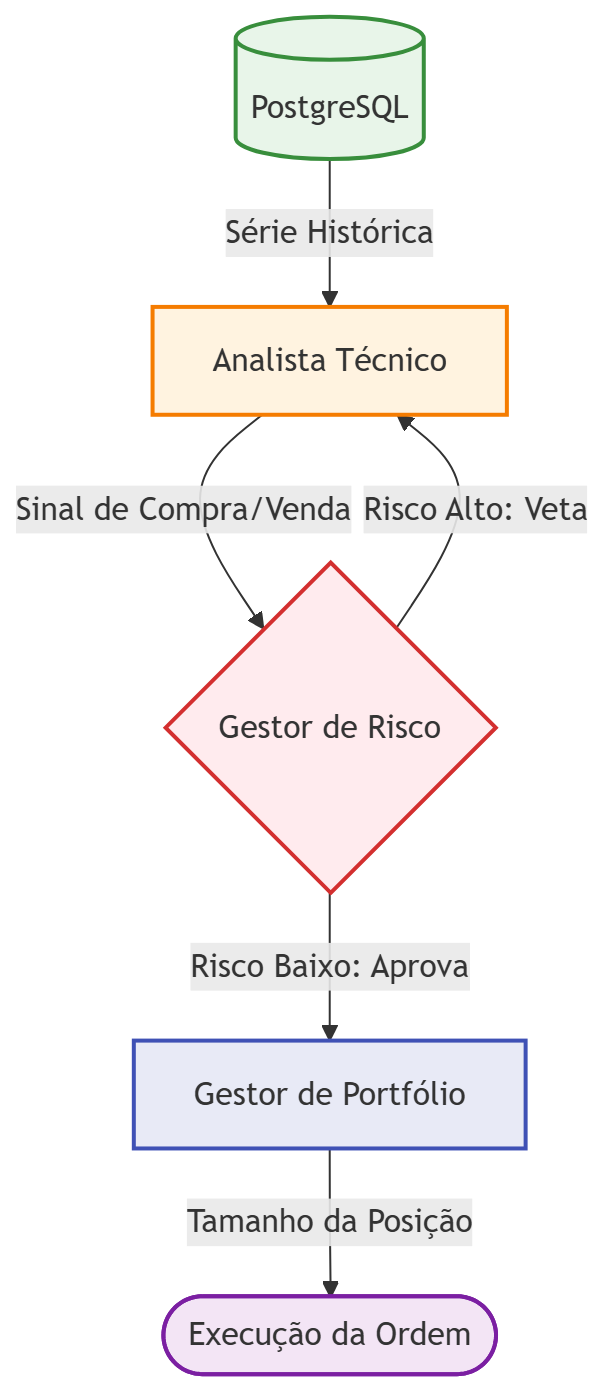
\includegraphics[height=9cm, keepaspectratio]{images/grafo-langgraph.png}
    \caption{Arquitetura do grafo de decisão e interação entre agentes no LangGraph.}
    \label{fig:grafo_agentes}
\end{figure}

\subsection{Fluxo de Consenso e Raciocínio}

Diferente de sistemas baseados em regras simples, esta arquitetura permite o raciocínio encadeado (\textit{Chain of Thought}). Ao encontrar uma anomalia nos dados da PETR4, por exemplo, o Gestor de Risco pode solicitar uma reavaliação ao Analista, simulando o comportamento de uma mesa de operações real. Esta abordagem visa mitigar falhas matemáticas puras através da supervisão qualitativa do LLM.

\section{ENGENHARIA DE PROMPT E DEFINIÇÃO DAS PERSONAS}

A eficácia de um sistema multiagente baseado em Large Language Models (LLMs) depende diretamente da qualidade da Engenharia de Prompt (\textit{Prompt Engineering}). Para o \textit{Hedge-fund-lab}, foi desenvolvida uma estrutura rigorosa de instruções visando garantir que cada agente assuma uma "persona" específica e limite sua análise aos dados numéricos fornecidos, mitigando o risco de alucinações.

A arquitetura define três agentes principais, cujos papéis e regras de instrução são:

\subsection{Agente Analista Técnico}
\begin{itemize}
    \item \textbf{Função:} Interpretar exclusivamente os indicadores matemáticos (Bandas de Bollinger, Médias Móveis Cruzadas, RSI e MACD).
    \item \textbf{Diretriz do Prompt:} O agente é instruído a ignorar notícias externas e focar apenas no cruzamento de sinais. A resposta deve ser estritamente categórica (COMPRA, VENDA ou MANTER) acompanhada de uma justificativa baseada na distância do preço atual em relação à média móvel ou aos desvios das Bandas de Bollinger.
\end{itemize}

\subsection{Agente Gestor de Risco}
\begin{itemize}
    \item \textbf{Função:} Atuar como um mecanismo de freio, protegendo o capital do fundo contra a volatilidade excessiva.
    \item \textbf{Diretriz do Prompt:} O agente recebe os sinais gerados pelo Analista Técnico e os cruza com métricas de risco, como o \textit{Maximum Drawdown} recente do ativo. Ele é instruído com limites rígidos (por exemplo, vetar qualquer operação de compra se a volatilidade do último mês exceder um teto predefinido), priorizando a preservação do caixa sobre o lucro potencial.
\end{itemize}

\subsection{Agente Gestor de Portfólio}
\begin{itemize}
    \item \textbf{Função:} Consolidar as visões técnicas e de risco e executar a decisão final.
    \item \textbf{Diretriz do Prompt:} Este agente opera como o árbitro final no grafo de decisão do LangGraph. Ele recebe o "estado" completo (o bloco de notas da reunião), pondera a confiança expressa pelos agentes anteriores e decide o dimensionamento da posição (\textit{Position Sizing}), determinando não apenas a direção da ordem, mas a quantidade de capital a ser alocada.
\end{itemize>


\chapter{Considerações Parciais e Metodologia}
\label{cha:resultados}

Este capítulo delineia os passos metodológicos que guiarão a fase prática da pesquisa (Projeto Final II), detalhando o planejamento experimental para a avaliação do sistema multiagente e o cronograma de atividades para a conclusão do trabalho.

\section{METODOLOGIA}

A presente pesquisa caracteriza-se como aplicada e de natureza quantitativa, adotando o método experimental por meio de simulação retrospectiva (\textit{backtesting}). O desenvolvimento da solução ocorrerá em três etapas principais: a construção do \textit{pipeline} de dados (ETL) e persistência no PostgreSQL; a implementação da arquitetura multiagente utilizando o \textit{framework} LangGraph e integração com as APIs de modelos de linguagem; e, por fim, a execução das simulações de investimento. O laboratório quantitativo (\textit{Hedge-fund-lab}) será testado sob condições simuladas do mercado real, permitindo a comparação direta de performance com algoritmos tradicionais.

\subsection{Planejamento do Experimento}

O experimento consistirá em submeter tanto as estratégias clássicas (Bandas de Bollinger e \textit{SMA Cross}) quanto o sistema multiagente a um período histórico de dez anos de dados de mercado da B3, especificamente avaliando os ativos PETR4 (cenário de alta volatilidade) e WEGE3 (cenário de tendência).

Para garantir a validade dos resultados e evitar o viés de \textit{data snooping}, o processo de avaliação seguirá o modelo \textit{out-of-sample}. O desempenho da carteira simulada não será medido apenas pelo lucro absoluto, mas pelas seguintes métricas financeiras ajustadas ao risco:
\begin{itemize}
    \item \textbf{Índice Sharpe e Índice Sortino:} Para avaliar se o retorno excedente justifica a volatilidade assumida pelo sistema ao longo do tempo.
    \item \textbf{\textit{Maximum Drawdown}:} Para medir a resiliência do Gestor de Risco em proteger o patrimônio durante crises sistêmicas ou quedas abruptas do ativo.
\end{itemize}

\subsection{Considerações Parciais}

Até a presente fase (Projeto Final I), foram consolidadas as bases teóricas do projeto, justificando a viabilidade técnica de utilizar \textit{Large Language Models} para emular comitês de investimento dinâmicos. O levantamento bibliográfico confirmou a relevância do problema, e a arquitetura de \textit{software} (modelagem relacional, orquestração de dados e roteamento de grafos) encontra-se plenamente desenhada. O foco da próxima etapa recairá exclusivamente sobre a programação dos artefatos computacionais e a coleta de resultados empíricos no laboratório quantitativo.

\subsection{Cronograma de Atividades}

Para a condução da segunda fase do projeto (Elaboração e Construção de Projeto Final), estabeleceu-se o seguinte cronograma de atividades, distribuído ao longo dos cinco meses letivos do próximo semestre:

\begin{table}[H]
\centering
\renewcommand{\arraystretch}{1.3}
\begin{tabularx}{\textwidth}{|X|c|c|c|c|c|}
\hline
\textbf{Atividades (TCC 2)} & \textbf{Mês 1} & \textbf{Mês 2} & \textbf{Mês 3} & \textbf{Mês 4} & \textbf{Mês 5} \\ \hline
Implementação do pipeline ETL e Banco de Dados & X & & & & \\ \hline
Desenvolvimento dos Agentes e LangGraph & & X & X & & \\ \hline
Execução do Backtesting e coleta de métricas & & & X & X & \\ \hline
Escrita da Avaliação Experimental (Cap. 4 - TCC 2) & & & & X & \\ \hline
Escrita da Conclusão, Revisão Final e Defesa & & & & & X \\ \hline
\end{tabularx}
\caption{Cronograma de atividades previsto para a conclusão do TCC}
\label{tab:cronograma}
\end{table}

%-----------------------------------------------
% Elementos Pós-Textuais
%-----------------------------------------------
\backmatter

\referencepage % Comando do molde para renderizar o arquivo "references.bib"

\end{document}